% 1977 年广东卷参考题 2：纸张矩形（左右长 x、上下宽 y），内阴影矩形为排版面 432，
% 左右边距 4 厘米、上下边距 3 厘米（按源卷第 5 页布局）
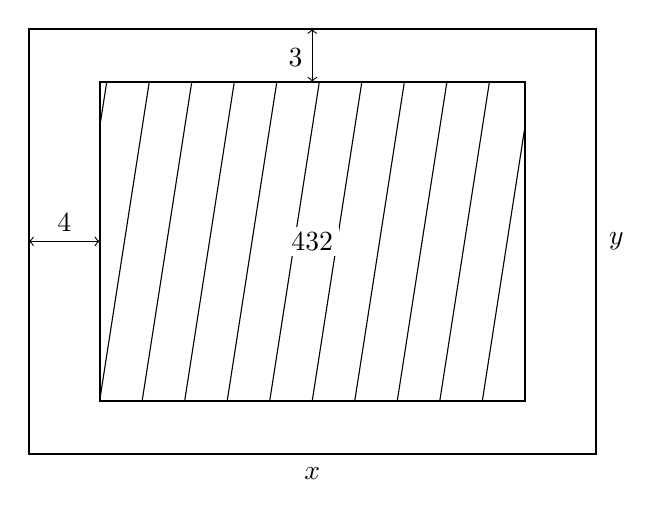
\begin{tikzpicture}[scale=0.9]
  \draw[thick] (0,0) rectangle (8,6);
  \begin{scope}
    \clip (1,0.75) rectangle (7,5.25);
    \foreach \i in {-7,...,10}
      \draw (1+\i*0.6,0.75) -- (1.7+\i*0.6,5.25);
  \end{scope}
  \draw[thick] (1,0.75) rectangle (7,5.25);
  \node[fill=white,inner sep=2pt] at (4,3) {$432$};
  % 边距标注
  \draw[<->] (0,3) -- (1,3);
  \node[above] at (0.5,3) {$4$};
  \draw[<->] (4,5.25) -- (4,6);
  \node[left] at (4,5.6) {$3$};
  % 纸张尺寸标注
  \node[below] at (4,-0.05) {$x$};
  \node[right] at (8.05,3) {$y$};
\end{tikzpicture}
